\documentclass[11pt,a4paper]{article}

\usepackage[margin=1.8cm]{geometry}
\usepackage{lmodern}
\usepackage[T1]{fontenc}
\usepackage[utf8]{inputenc}
\usepackage{amsmath,amssymb,mathtools}
\usepackage{booktabs,array,tabularx,longtable}
\usepackage{enumitem}
\usepackage{xcolor}
\usepackage[most]{tcolorbox}
\usepackage{tikz}
\usepackage{fancyhdr}
\usepackage{titlesec}
\usepackage{setspace}
\usepackage{microtype}
\usepackage{hyperref}

\hypersetup{
  colorlinks=true,
  linkcolor=blue!50!black,
  urlcolor=blue!50!black,
  pdftitle={PYL7167 Atomic Physics Quiz Notes},
  pdfauthor={Quiz study pack}
}

\definecolor{ink}{HTML}{1A1A1A}
\definecolor{boxbg}{HTML}{F4F7FB}
\definecolor{boxbd}{HTML}{2C5F8A}
\definecolor{warnbg}{HTML}{FFF6E5}
\definecolor{warnbd}{HTML}{B86E00}
\definecolor{okbg}{HTML}{EAF6EE}
\definecolor{okbd}{HTML}{1B6B3A}

\tcbset{
  common/.style={
    enhanced,
    colback=boxbg,
    colframe=boxbd,
    boxrule=0.6pt,
    arc=2pt,
    left=8pt,right=8pt,top=5pt,bottom=5pt,
    fontupper=\normalsize
  }
}
\newtcolorbox{keybox}[1][]{common, title={#1}, coltitle=white, colbacktitle=boxbd, attach boxed title to top left={yshift=-2mm,xshift=4mm}, boxed title style={arc=1pt}}
\newtcolorbox{trapbox}{common, colback=warnbg, colframe=warnbd}
\newtcolorbox{ansbox}{common, colback=okbg, colframe=okbd}

\pagestyle{fancy}
\fancyhf{}
\fancyhead[L]{\small PYL7167 / AMP 7167 \textemdash{} Atomic Physics Quiz}
\fancyhead[R]{\small Study notes}
\fancyfoot[C]{\thepage}
\renewcommand{\headrulewidth}{0.4pt}

\titleformat{\section}{\large\bfseries\color{boxbd}}{\thesection}{0.6em}{}
\titleformat{\subsection}{\normalsize\bfseries\color{boxbd!80!black}}{\thesubsection}{0.5em}{}
\titlespacing*{\section}{0pt}{12pt}{6pt}
\titlespacing*{\subsection}{0pt}{8pt}{4pt}
\setlist[itemize]{leftmargin=1.3em,itemsep=2pt,topsep=3pt}
\setlist[enumerate]{leftmargin=1.5em,itemsep=2pt,topsep=3pt}
\setstretch{1.08}

\newcommand{\term}[1]{\ensuremath{{}^{#1}}}
\DeclareMathOperator{\eV}{eV}

\begin{document}
\thispagestyle{plain}

\begin{center}
{\LARGE\bfseries PYL7167 / AMP 7167}\\[4pt]
{\Large Atomic Physics --- Quiz Study Notes}\\[8pt]
{\large Readable PDF: formulae, theory, and all 18 practice solutions}\\[6pt]
\small From your lecture notes, the practice set (high emphasis), and Haken \& Wolf, Bransden \& Joachain, White, Foot, Kittel, Jackson.
\end{center}

\vspace{6pt}
\begin{trapbox}
\textbf{How to use this file tonight.}
\begin{enumerate}
  \item Memorise Part~I (formula sheet), 30 minutes.
  \item Skim Part~II only on topics you are weak on.
  \item Work Part~III on paper first, then check. Do not skip 9, 11, 12, 15, 17, 18.
  \item In the morning, read only Part~IV.
\end{enumerate}
If you have two hours: Part~I, problems 1--8 and 18, then diagrams in 9, 12, 16, then Part~IV.
\end{trapbox}

\tableofcontents
\newpage

%======================================================================
\section{Formula sheet}
%======================================================================

\subsection*{Constants to memorise}
\begin{keybox}{Use these unless the paper gives others}
\[
\begin{aligned}
R_\infty &= 109\,737.318~\mathrm{cm}^{-1}, &
R_H &\approx 109\,677.6~\mathrm{cm}^{-1},\\
hcR_\infty &= 13.6~\mathrm{eV}, &
a_0 &= 0.529~\text{\AA},\\
\alpha &= 1/137, &
c &= 137~\mathrm{a.u.},\\
\mu_B &= e\hbar/2m_e, &
m_p/m_e &\approx 1836,\\
M_D/m_e &\approx 3670, &
k_B &= 8.617\times 10^{-5}~\mathrm{eV\,K}^{-1}.
\end{aligned}
\]
Sodium D lines: \(D_2\): \(3\,{}^2P_{3/2}\to 3\,{}^2S_{1/2}\) at \textbf{589.0 nm};
\(D_1\): \(3\,{}^2P_{1/2}\to 3\,{}^2S_{1/2}\) at \textbf{589.6 nm}.
\end{keybox}

\subsection{Hydrogenic energies and spectra}

Bohr / Schr\"odinger energy (reduced mass \(\mu\)):
\[
E_n = -\frac{\mu Z^2 e^4}{2(4\pi\epsilon_0)^2\hbar^2}\,\frac{1}{n^2}
= -\,13.6~\mathrm{eV}\cdot\frac{\mu}{m_e}\cdot\frac{Z^2}{n^2}.
\]
Rydberg formula:
\[
\frac{1}{\lambda} = R_M Z^2\left(\frac{1}{n_f^2}-\frac{1}{n_i^2}\right),\qquad
R_M = R_\infty\frac{\mu}{m_e} = \frac{R_\infty}{1+m_e/M},
\]
\[
R_\infty = \frac{m_e e^4}{8\varepsilon_0^2 h^3 c} = 109\,737.318~\mathrm{cm}^{-1}.
\]
Series limit (\(n_i\to\infty\)): \(1/\lambda_\infty = R_M Z^2/n_f^2\).
Longest wavelength in a series: \(n_i=n_f+1\). Shortest = series limit.

\begin{center}
\small
\begin{tabular}{@{}lllll@{}}
\toprule
Series & \(n_f\) & \(\lambda\) range (H) & Region & Overlap? \\
\midrule
Lyman    & 1 & 91.2--121.6 nm  & UV            & no overlap with Balmer \\
Balmer   & 2 & 364.6--656.3 nm & vis \(\to\) near UV & no overlap with Paschen \\
Paschen  & 3 & 820.4--1875 nm  & IR            & \textbf{overlaps Brackett} \\
Brackett & 4 & 1458--4051 nm   & IR            & \textbf{overlaps Paschen and Pfund} \\
Pfund  & 5 & 2279--7460 nm   & IR            & \textbf{overlaps Brackett} \\
\bottomrule
\end{tabular}
\end{center}

Correspondence principle (\(n\gg 1\), \(\Delta n=p\) small):
\[
\frac{1}{\lambda}\approx (\text{const})\frac{p}{n^3},\qquad
\omega_{\mathrm{orb}}=2\pi\cdot 2Rc/n^3.
\]
Equating classical \(E(\omega)\) to \(E_n=-Rch/n^2\) recovers \(R_\infty\).

Exotic atoms / excitons --- same formulae with the actual reduced mass and dielectric constant:
\[
\mu_{\pi p}=\frac{m_\pi m_p}{m_\pi+m_p},\qquad
R_{\mathrm{ex}}=\frac{13.6~\mathrm{eV}}{\varepsilon_r^2}\frac{\mu}{m_e}.
\]
Wannier exciton: \(E_n=E_g-R_{\mathrm{ex}}/n^2\). Absorption: hydrogen-like discrete lines plus continuum for \(h\nu>E_g\).

\subsection{Atomic units, sizes, virial}
\[
a_0=0.529~\text{\AA},\quad
1~\text{Hartree}=27.2~\mathrm{eV}=2\times 13.6~\mathrm{eV},\quad
v_1=\alpha c=c/137.
\]
\[
\langle r\rangle_{nlm}=\frac{a_0 n^2}{Z}\left\{1+\frac12\left[1-\frac{\ell(\ell+1)}{n^2}\right]\right\},
\qquad
\left\langle\frac1r\right\rangle_{nlm}=\frac{Z}{a_\mu n^2}.
\]
Most probable radius \(\neq\langle r\rangle\) (the radial tail pulls \(\langle r\rangle\) out).
For 1s: \(r_{\mathrm{mp}}=a_0/Z\), \(\langle r\rangle=1.5\,a_0/Z\).
Rydberg atom: \(r_n=n^2 a_0\), \(E_b=13.6~\mathrm{eV}/n^2\), \textbf{weakly} bound.

Virial for \(V=\alpha r^k\): \(2\langle T\rangle=k\langle V\rangle\).
Coulomb \(k=-1\): \(\langle T\rangle=-E\), \(\langle V\rangle=2E\).
Harmonic oscillator \(k=2\): \(\langle T\rangle=\langle V\rangle\).

Small-\(r\) radial behaviour: \(R_{nl}(r)\propto r^{\ell}\) (the function \(u=rR\propto r^{\ell+1}\)).

Unsold: \(\sum_{m=-\ell}^{\ell}|Y_{\ell m}|^2=(2\ell+1)/4\pi\) (angle-independent). Closed shells are spherically symmetric.

\subsection{Alkali atoms and quantum defect}
The central field is still spherical (so \(m\) remains degenerate) but \textbf{not} pure Coulomb, so \(\ell\)-degeneracy dies.
\[
E_{n\ell}=-R\,hc\big/\bigl(n-\delta_{n\ell}\bigr)^2.
\]
Penetration: \(\delta_s\gg\delta_p\gg\delta_d\approx\delta_f\approx 0\).
For Li (your notes): \(\delta_s\approx 0.4\), \(\delta_p\approx 0.04\), \(\delta_{d,f}\approx 0\).
Ground state of Li: \(1s^2 2s\;{}^2S_{1/2}\). Resonance line \(2p\to 2s\).
Why \(\ell<n\): radial quantum number \(n_r=n-\ell-1\ge 0\).

\subsection{Angular momentum, terms, coupling}
\[
\mathbf{J}=\mathbf{L}+\mathbf{S},\qquad
\mathbf{L}\cdot\mathbf{S}=\frac12\bigl(J^2-L^2-S^2\bigr).
\]
Term symbol: \({}^{2S+1}L_J\) with \(L=S,P,D,F,\ldots\) (\(L=0,1,2,3,\ldots\)).

\textbf{LS} (light atoms): \(\mathbf{L}=\sum\mathbf{l}_i\), \(\mathbf{S}=\sum\mathbf{s}_i\), then \(\mathbf{J}=\mathbf{L}+\mathbf{S}\).\\
\textbf{jj} (heavy atoms): \(\mathbf{j}_i=\mathbf{l}_i+\mathbf{s}_i\), then \(\mathbf{J}=\sum\mathbf{j}_i\).

Two nonequivalent electrons \(\ell_1=1\), \(\ell_2=2\):
\(L=1,2,3\), \(S=0,1\) \(\Rightarrow\) \({}^1P,{}^1D,{}^1F,{}^3P,{}^3D,{}^3F\),
with \(J=|L-S|\ldots L+S\).

Hund (LS, equivalent electrons): (1)~max \(S\); (2)~then max \(L\); (3)~ \(J_{\min}\) if shell \(<\) half full, \(J_{\max}\) if \(>\) half full.

jj equivalent electrons \(j=5/2\):
\[
(5/2)^{1,5}:\;J=5/2;\quad
(5/2)^{2,4}:\;J=0,2,4;\quad
(5/2)^3:\;J=3/2,5/2,9/2;\quad
(5/2)^6:\;J=0.
\]
Hole--particle: \((j)^{2j+1-N}\) has the same \(J\) list as \((j)^N\).

Magnetic moment (weak \(B\)):
\[
\boldsymbol{\mu}_J=-g_J\mu_B\mathbf{J}/\hbar,\qquad
g_J=1+\frac{J(J+1)+S(S+1)-L(L+1)}{2J(J+1)},
\]
\[
\mu=g_J\sqrt{J(J+1)}\,\mu_B,\qquad
\Delta E=g_J\mu_B B m_J.
\]
\(g_L=1\), \(g_S=2.0023\approx 2\). Gyromagnetic: \(\omega_L=\gamma B\), \(\gamma_L=e/2m\), \(\gamma_S\approx e/m\).

Helium: para \(S=0\) (singlets, including GS \(1s^2\;{}^1S_0\)); ortho \(S=1\) (triplets). Intercombination lines are E1-forbidden \(\Rightarrow\) two superimposed spectra.

\subsection{Fine structure (spin--orbit)}
Internal \(\mathbf{B}\) of orbital motion + Thomas factor \(1/2\):
\[
V_{LS}=\frac{Ze^2\mu_0}{8\pi m_e^2 r^3}\,\mathbf{S}\cdot\mathbf{L}
=\frac{a}{2}\bigl[j(j+1)-\ell(\ell+1)-s(s+1)\bigr],
\]
\[
\left\langle\frac1{r^3}\right\rangle=\frac{Z^3}{a_H^3 n^3 \ell(\ell+\tfrac12)(\ell+1)}\qquad(\ell\ge 1).
\]
Interval between \(j=\ell+\tfrac12\) and \(j=\ell-\tfrac12\):
\[
\Delta E_{\mathrm{fs}}\propto\frac{Z^4}{n^3\,\ell(\ell+1)}.
\]
Dirac / rel.\ QM: \(E=E(n,j)\) not \(E(n,\ell)\).
Lamb shift (QED) splits \(2S_{1/2}\) \textbf{above} \(2P_{1/2}\) by \(1057.8~\mathrm{MHz}\approx 0.035~\mathrm{cm}^{-1}\)
(this is \textbf{not} \(0.031~\mathrm{eV}\)).
\(2S_{1/2}\) is metastable (E1 \(2S\to 1S\) forbidden, \(\Delta\ell=0\)).

\subsection{External fields}

\textbf{Stern--Gerlach.}
\[
U=-\boldsymbol{\mu}\cdot\mathbf{B},\qquad
F_z\approx\mu_z\frac{\partial B_z}{\partial z}.
\]
\(^{2}S_{1/2}\) alkali: 2 beams, \(\mu_z=\pm\mu_B\). Cannot be done with free electrons (Lorentz force swamps the spin force).
Deflection of one component after magnet length \(L\) plus drift \(\ell\), speed \(v\):
\[
s=\frac{\mu_z}{M}\frac{\partial B_z}{\partial z}\frac{L}{v^2}\left(\ell+\frac{L}{2}\right),\qquad
\text{spot separation }=2s.
\]
Use \(v=\sqrt{2kT/M}\) unless told otherwise.

\textbf{Zeeman Hamiltonian.}
\[
H'=\frac{\mu_B}{\hbar}(\mathbf{L}+2\mathbf{S})\cdot\mathbf{B}=\mu_B B(L_z+2S_z)/\hbar.
\]
\begin{center}
\small
\begin{tabular}{@{}llll@{}}
\toprule
Regime & Criterion & Energies & Pattern \\
\midrule
Weak / anomalous & \(\mu_B B\ll E_{\mathrm{fs}}\) & \(g_J\mu_B B m_J\) & many uneven components \\
Normal & \(S=0\) so \(g=1\) & \(\mu_B B m_L\) & Lorentz triplet \\
Paschen--Back & \(\mu_B B\gg E_{\mathrm{fs}}\) & \(\mu_B B(m_L+2m_S)\) & normal triplet restored \\
\bottomrule
\end{tabular}
\end{center}
E1 selection: \(\Delta m_J=0\) (\textbf{\(\pi\)}, linear \(\parallel\mathbf{B}\)),
\(\Delta m_J=\pm 1\) (\textbf{\(\sigma\)}, circular about \(\mathbf{B}\)).
Also \(\Delta J=0,\pm 1\) (not \(0\to 0\)), \(\Delta L=\pm 1\), \(\Delta S=0\), and \(\Delta m_S=0\) in Paschen--Back.

Land\'e \(g\) values you will need:
\begin{center}
\begin{tabular}{@{}lc@{}}
\toprule
Term & \(g_J\) \\
\midrule
\({}^2S_{1/2}\) & 2 \\
\({}^2P_{1/2}\) & \(2/3\) \\
\({}^2P_{3/2}\) & \(4/3\) \\
\({}^2D_{3/2}\) & \(4/5\) \\
\({}^2D_{5/2}\) & \(6/5\) \\
\({}^1P_1,{}^1D_2\) (singlets) & 1 \\
\bottomrule
\end{tabular}
\end{center}

\textbf{Linear Stark} (hydrogen only, first order) because of \(\ell\)-degeneracy:
\[
\Delta E=\frac32 n(n_1-n_2)\,e a_0\,\mathcal{E},\qquad n=n_1+n_2+|m|+1.
\]
\(n=2\): three levels, \(\Delta E=0,\pm 3\,e a_0\mathcal{E}\).
\(n=3\): five levels, \(\Delta E=0,\pm\tfrac92 e a_0\mathcal{E},\pm 9\,e a_0\mathcal{E}\).
Alkali / non-H: only \textbf{quadratic} Stark.
Polarisation: \(\pi\) if \(\Delta m=0\), \(\sigma\) if \(\Delta m=\pm 1\).

\subsection{Radiation, Einstein, selection rules}
Semiclassical: field classical, atom quantum. Coulomb gauge \(\nabla\cdot\mathbf{A}=0\).
\[
H=\frac1{2m}(\mathbf{p}+e\mathbf{A})^2+V.
\]
Drop \(A^2\) at low intensity (keeping it gives multiphoton processes).
Dipole (E1): \(e^{i\mathbf{k}\cdot\mathbf{r}}\approx 1\), rate \(\propto|\hat{\epsilon}\cdot\mathbf{r}_{ba}|^2\).

E1 selection:
\[
\Delta \ell=\pm 1,\quad \Delta m=0,\pm 1,\quad \Delta S=0,\quad
\Delta J=0,\pm 1\ (J=0\not\to J=0),\quad \text{parity changes.}
\]
\(\Delta m=0\): linear (\(z\), \(\pi\)). \(\Delta m=\pm 1\): circular (\(\sigma_\pm\), \(x\pm iy\)).
Dipole-forbidden \(\neq\) strictly forbidden (M1, E2, two-photon, collisions).

Einstein (energy density per Hz):
\[
A_{21}=\frac{8\pi h\nu^3}{c^3}B_{21},\qquad B_{12}=\frac{g_2}{g_1}B_{21}.
\]
Stimulated rate \(\propto\) intensity. Spontaneous \(A\) is not.

Natural (Lorentzian) FWHM of a line to a stable lower level:
\[
\Delta E=\hbar/\tau,\qquad \Delta\nu=\frac{1}{2\pi\tau},\qquad
\Delta\lambda=\frac{\lambda^2}{c}\Delta\nu.
\]
\(\tau=\) \textbf{mean} life. If half-life is given, \(\tau=t_{1/2}/\ln 2\).

\subsection{Line shapes}
Doppler (Gaussian) FWHM:
\[
\Delta\nu_D=\frac{2\nu_0}{c}\sqrt{\frac{2kT\ln 2}{M}},\qquad
\Delta\lambda_D=\frac{2\lambda_0}{c}\sqrt{\frac{2kT\ln 2}{M}},
\]
\[
I(\nu)=I(\nu_0)\exp\left[-\frac{Mc^2}{2kT}\left(\frac{\nu-\nu_0}{\nu_0}\right)^2\right].
\]
Doppler \textbf{shift} of one velocity class: \(\Delta\nu/\nu=v/c\). Doppler \textbf{width} is the FWHM of the thermal envelope.
Pressure broadening: collisions, can be asymmetric, and shortens lifetime.

\subsection*{Lecture side-notes}
\begin{itemize}
\item Optical electron = valence electron that is excited. Equivalent electrons share \((n,\ell)\).
\item Line spectra: atoms. Band: molecules/solids. Continuous: black-body / free--bound.
\item Photocell: reverse-biased pn, \(h\nu>E_g\). Solar cell: same physics, \textbf{no} bias.
\item Auger kinetic energy is a difference of binding energies; independent of the photon that dug the hole.
\item King: \(|q_p+q_e|\lesssim 10^{-20}e\).
\item Classical radiative collapse of H: Larmor, \(T\sim 10^{-11}\,\mathrm{s}\) (not ms).
\item Relativistic mass correction to \(R\) is not enough for \(Z\gtrsim 20\).
\end{itemize}

\newpage
%======================================================================
\section{Theory notes}
%======================================================================

\subsection{What an ``atom'' means in this course}
\textbf{One-electron (hydrogenic) atoms:} a nucleus of charge \(+Ze\) plus exactly one electron.
Examples: H, \(\mathrm{He}^+\), \(\mathrm{Li}^{2+}\), \(\mathrm{C}^{5+}\). Energies scale as \(Z^2\), lengths as \(1/Z\).

\textbf{Optical (valence) electrons:} the electrons that actually change state in optical spectra. Na has one; Ca has two.

\textbf{Equivalent electrons:} same \(n\) and \(\ell\). Helium \(1s^2\) is two equivalent \(s\) electrons.

Three kinds of spectra: \textbf{line} (atoms), \textbf{band} (molecules/solids), \textbf{continuous} (free--bound or black-body).

Helium looks like two superimposed spectra: \emph{parahelium} (singlets, \(S=0\), includes the ground state \(1s^2\;{}^1S_0\)) and \emph{orthohelium} (triplets, \(S=1\), lowest term \(1s2s\;{}^3S_1\), metastable). E1 cannot change \(S\).

\subsection{Bohr model, Rydberg constant, correspondence principle}
Classical circular orbit: Coulomb = centripetal
\[
\frac{1}{4\pi\epsilon_0}\frac{e^2}{r^2}=m r\omega^2
\quad\Rightarrow\quad
E=T+V=-\frac12\cdot\frac{e^2}{4\pi\epsilon_0 r}.
\]
Eliminating \(r\) in favour of \(\omega\):
\[
E=-\frac12(4\pi\epsilon_0)^{-2/3}(e^4 m\omega^2)^{1/3}.
\]
Quantum frequencies of neighbouring levels at large \(n\):
\[
\nu=Rc\left(\frac{1}{n^2}-\frac{1}{(n+1)^2}\right)\approx 2Rc/n^3,\qquad\omega=2\pi\nu.
\]
Match \(E_n=-Rch/n^2\) to the classical \(E(\omega)\) and you recover \(R_\infty=m_e e^4/(8\varepsilon_0^2 h^3 c)\).

Experiment: \(R_H=109\,677.58~\mathrm{cm}^{-1}\). Infinite-mass theory: \(R_\infty=109\,737.32~\mathrm{cm}^{-1}\).
The gap \(\approx 60~\mathrm{cm}^{-1}\) is \textbf{reduced mass}:
\[
R_H=\frac{R_\infty}{1+m_e/M_p}.
\]
This fix is not enough for \(Z\gtrsim 20\): fine structure and QED grow as \(Z^4\) and higher.

Resonance line of H: Lyman-\(\alpha\), \(n=2\to 1\), \(121.6~\mathrm{nm}\).

Classical collapse (Larmor): an accelerating charge radiates \(P=\mu_0 e^2 a^2/(6\pi c)\). Time to spiral from \(a_0\) into the nucleus is \(\sim 10^{-11}\,\mathrm{s}\) --- not milliseconds. Bohr stops this by forbidding continuous radiation in a stationary state.

\subsection{Schr\"odinger hydrogen: degeneracy, radial functions, virial}
Central potential \(\Rightarrow\) \([H,\mathbf{L}]=[H,L^2]=0\), so \(\{H,L^2,L_z\}\) share eigenfunctions
\[
\psi_{nlm}(\mathbf{r})=R_{nl}(r)\,Y_{\ell m}(\theta,\phi).
\]
\begin{itemize}
\item Energy of a pure Coulomb problem depends only on \(n\) (\textbf{accidental / \(\ell\)-degeneracy}), degeneracy \(n^2\) without spin, \(2n^2\) with spin.
\item \(m\)-degeneracy is from \textbf{spherical symmetry} (any central \(V(r)\)). It survives in alkalis; \(\ell\)-degeneracy does not.
\end{itemize}
Why \(\ell<n\): bound Coulomb solutions exist only for \(n_r=0,1,2,\ldots\) with \(n=n_r+\ell+1\).

Near the origin: \(R_{nl}(r)\to r^{\ell}\). (\(u=rR\propto r^{\ell+1}\). If a T/F says ``\(R_{nl}\propto r^{\ell+1}\)'', it is false.)

Useful functions:
\[
R_{10}(r)=2\left(\frac{Z}{a_0}\right)^{3/2}e^{-Zr/a_0},\qquad
R_{21}(r)=\frac{1}{\sqrt{3}}\left(\frac{Z}{2a_0}\right)^{3/2}\left(\frac{Zr}{a_0}\right)e^{-Zr/2a_0}.
\]
Larger \(Z\) pulls \(|R|^2\) inward. \(s\) waves have \(R(0)\neq 0\) (electron capture possible).

Radial probability \(P(r)=r^2|R_{nl}|^2\). Maxima from \(dP/dr=0\), not from \(\langle r\rangle\). \(\langle r\rangle>r_{\mathrm{mp}}\) because \(P(r)\) has a long outer tail.

Virial: Coulomb \(\langle T\rangle=+13.6~\mathrm{eV}\), \(\langle V\rangle=-27.2~\mathrm{eV}\), \(E=-13.6~\mathrm{eV}\) for H 1s.

Unsold's theorem: a closed subshell is spherically symmetric. Proof for \(\ell=1\) is problem~17.

\subsection{Alkali atoms, quantum defect, ionisation}
An alkali is hydrogen-like \textbf{outside} a closed noble-gas core. The valence electron sees \(V\sim -e^2/4\pi\epsilon_0 r\) far away (core charge \(+1\)), and \(V\sim -Ze^2/4\pi\epsilon_0 r\) if it penetrates the core.

\begin{trapbox}
Do \textbf{not} write ``the potential is not spherically symmetric''. That would split \(m\), which it does not. Spherical symmetry is intact; Coulomb degeneracy is not.
\end{trapbox}

Quantum defect \(\delta_{n\ell}\) absorbs core penetration and polarisation:
\[
E_{n\ell}=-R_{\mathrm{atom}}hc\big/(n-\delta_{n\ell})^2,\qquad n^*=n-\delta.
\]
\(\delta\) is nearly independent of \(n\) for a given \(\ell\), and falls rapidly with \(\ell\).

Term diagram vs hydrogen: every \(ns\) level of Li sits \textbf{below} the H level of the same \(n\); \(np\) slightly below; \(nd,nf\) almost on top of H. Ground state is \(2s\), not \(1s\). Allowed arrows: \(\Delta\ell=\pm 1\).

Ionisation energies jump when you start breaking a closed shell (Li: \(5.4~\mathrm{eV}\) then \(\sim 75~\mathrm{eV}\)).

\subsection{Fine structure, relativistic QM, Lamb shift}
In the electron's rest frame the nucleus orbits, producing \(\mathbf{B}_L\propto\mathbf{L}/r^3\). Then \(V=-\boldsymbol{\mu}_s\cdot\mathbf{B}_L\) with a Thomas factor \(1/2\). On \(\lvert n\ell jm_j\rangle\),
\[
\mathbf{L}\cdot\mathbf{S}=\frac{\hbar^2}{2}\bigl[j(j+1)-\ell(\ell+1)-s(s+1)\bigr],
\]
so each Bohr level with \(\ell\ge 1\) splits into \(j=\ell\pm\tfrac12\). The doublet interval scales as \(Z^4/[n^3\ell(\ell+1)]\).

Hydrogen \(2p\) interval is \(0.365~\mathrm{cm}^{-1}\) (\(\sim 4.5\times 10^{-5}\,\mathrm{eV}\)). A problem that quotes ``\(0.3~\mathrm{eV}\)'' is a \textbf{scaling exercise}, not a measured number.

Dirac hydrogen: \(E=E(n,j)\). Thus \(2S_{1/2}\) and \(2P_{1/2}\) are still degenerate. Lamb--Retherford (1947): microwave resonance on a hot H beam; \(2S_{1/2}\) is metastable and survives a \(10~\mathrm{cm}\) flight; extrapolate to \(B=0\). Result: \(2S_{1/2}\) lies \textbf{\(1057.8~\mathrm{MHz}\) above} \(2P_{1/2}\). This is a QED radiative correction, not predicted by Dirac. Frequency \(1057~\mathrm{MHz}\approx 4.4~\mu\mathrm{eV}\approx 0.035~\mathrm{cm}^{-1}\). If lecture notes say ``\(0.031~\mathrm{eV}\)'', that is a unit slip.

Metastable \(2S_{1/2}\) of H: E1 needs \(\Delta\ell=\pm 1\); there is no lower \(\ell=1\) state below \(2S\). Decay is two-photon, lifetime \(\sim 0.12\,\mathrm{s}\). (\(2P\) lives \(1.6~\mathrm{ns}\).)

\subsection{Magnetic moments, Larmor, Stern--Gerlach}
Orbital: \(\boldsymbol{\mu}_L=-(e/2m_e)\mathbf{L}\), \(g_L=1\).
Spin: \(\boldsymbol{\mu}_S=-g_S\mu_B\mathbf{S}/\hbar\), \(g_S\approx 2\).
Because \(g_S\neq g_L\), \(\boldsymbol{\mu}_J\) is not simply antiparallel to \(\mathbf{J}\); the surviving projection is the Land\'e one.

Torque \(\boldsymbol{\tau}=\boldsymbol{\mu}\times\mathbf{B}\) \(\Rightarrow\) Larmor precession \(\omega_L=\gamma B\), independent of the angle \(\alpha\) between \(\boldsymbol{\mu}\) and \(\mathbf{B}\).

SG force in an inhomogeneous field: \(\mathbf{F}=\nabla(\boldsymbol{\mu}\cdot\mathbf{B})\). With the standard pole-piece geometry, \(F_z=\mu_z\partial B_z/\partial z\). Alkali GS \({}^2S_{1/2}\): two spots. A \(J=3/2\) beam would give four spots. Free electrons fail because of \(e\mathbf{v}\times\mathbf{B}\). Use neutral atoms (Ag, Cu, H, Na, K, Cs).

\subsection{Zeeman, Paschen--Back, and Stark}
Full magnetic Hamiltonian (one electron, ignoring diamagnetism):
\[
H=H_0+\zeta\,\mathbf{L}\cdot\mathbf{S}+\frac{\mu_B}{\hbar}(\mathbf{L}+2\mathbf{S})\cdot\mathbf{B}.
\]
``Weak'' vs ``strong'' is relative to the internal FS interval of that atom.

\textbf{Normal Zeeman} (\(S=0\), e.g.\ Cd \({}^1D_2\to{}^1P_1\)): \(g=1\) on both levels. Selection \(\Delta m=0,\pm 1\) yields the Lorentz triplet.

\textbf{Anomalous Zeeman} (\(S\neq 0\)): each FS level fans into \(2J+1\) sublevels with spacing \(g_J\mu_B B\). Because \(g_{\mathrm{upper}}\neq g_{\mathrm{lower}}\), you get many components with unequal spacing. Sodium D: \(D_2={}^2P_{3/2}\to{}^2S_{1/2}\) (stronger); \(D_1={}^2P_{1/2}\to{}^2S_{1/2}\).

\textbf{Paschen--Back:} \(\mathbf{L}\) and \(\mathbf{S}\) decouple. Good quantum numbers \(m_L,m_S\). Energies \(E=\mu_B B(m_L+2m_S)\). Optical selection \(\Delta m_L=0,\pm 1\), \(\Delta m_S=0\) collapses the forest back to a normal triplet.

\textbf{Stark:} \(H'=e\mathcal{E}z\). Hydrogen has a \textbf{linear} (first-order) Stark effect because of \(\ell\)-degeneracy. Non-hydrogenic atoms have only quadratic Stark (\(\langle z\rangle=0\) by parity). Polarisation: \(\pi\) (\(\Delta m=0\)) and \(\sigma\) (\(\Delta m=\pm 1\)).

\subsection{Interaction with light}
Treat \(\mathbf{E},\mathbf{B}\) classically and the atom quantum-mechanically.
\[
i\hbar\partial_t\Psi=\left[\frac{1}{2m}(-i\hbar\nabla+e\mathbf{A})^2+V(r)\right]\Psi.
\]
Identify \(H_0=p^2/2m+V\) and \(H'\approx (e/m)\mathbf{A}\cdot\mathbf{p}\). First-order TDPT, long-time limit, produces a rate \(\propto\) (intensity) \(\times|M_{ba}|^2\).

Dipole approximation: \(\lambda\gg a_0\), so \(e^{i\mathbf{k}\cdot\mathbf{r}}\approx 1\) and \(M\propto\hat\epsilon\cdot\mathbf{r}_{ba}\). Angular integrals of \(z=r\cos\theta\) force \(\Delta m=0\); \(x\pm iy\) force \(\Delta m=\pm 1\). Parity of \(Y_{\ell m}\) is \((-1)^\ell\), so E1 changes parity.

Einstein \(A\) (spontaneous) is not in semiclassical Maxwell theory; QM derives \(B\), then \(A_{21}=(8\pi h\nu^3/c^3)B_{21}\). Absorption and stimulated emission share the same \(|M|^2\). Scattering is a second-order two-photon process; absorption is first-order.

\subsection{Widths and shapes}
An excited state with mean life \(\tau\) is not monochromatic: \(\Delta E\,\Delta t\sim\hbar\) with \(\Delta t\sim\tau\).

\begin{center}
\small
\begin{tabular}{@{}llll@{}}
\toprule
Mechanism & Shape & Scales as & Notes \\
\midrule
Natural & Lorentzian & \(1/\tau\) & homogeneous; independent of \(T\) \\
Doppler & Gaussian & \(\sqrt{T/M}\,\nu_0\) & inhomogeneous; thermal \(v_x\) \\
Pressure / collision & often Lorentzian, can be asymmetric & density \(\times\sigma\times v\) & shortens effective \(\tau\) \\
\bottomrule
\end{tabular}
\end{center}
Rule of thumb: optical Doppler at 300~K is GHz; natural is MHz (Na \(D_2\): \(\tau=16~\mathrm{ns}\Rightarrow\Delta\nu\approx 10~\mathrm{MHz}\)).

\subsection{Multi-electron bookkeeping}
LS coupling (light atoms, residual Coulomb \(\gg\) spin--orbit): Pauli-allowed \((S,L)\) terms, then \(J=|L-S|\ldots L+S\), then Hund.

jj coupling (heavy atoms): each electron has a good \(j=\ell\pm 1/2\); equivalent-\(j\) occupations restricted by Pauli on \(m_j\). Use hole--particle symmetry.

Platinum \([\mathrm{Xe}]4f^{14}5d^9 6s^1\): a \(d\)-hole plus an \(s\) electron \(\Rightarrow\) \({}^3D\) and \({}^1D\). More-than-half \(d^9\) \(\Rightarrow\) inverted FS, GS \({}^3D_3\). Then \(g=4/3\), \(\mu=(8\sqrt{3}/3)\mu_B\), weak-field span \(=8\mu_B B\).

Helium spin: the triplet \(S=1\) subspace is \(\{\lvert\uparrow\uparrow\rangle,\;(\lvert\uparrow\downarrow\rangle+\lvert\downarrow\uparrow\rangle)/\sqrt{2},\;\lvert\downarrow\downarrow\rangle\}\). Problem 15 is the \(\lvert\downarrow\downarrow\rangle\) case done with Pauli matrices.

\subsection{Lecture odds and ends}
\textbf{Photocell vs solar cell.} Both: \(h\nu>E_g\) creates \(e\)--\(h\) pairs at a pn junction. Photocell is reverse biased. Solar cell has no bias.

\textbf{Faraday cup.} Measures beam current. A suppressor electrode throws secondary electrons back into the cup.

\textbf{Auger / Coster--Kronig.} A core hole is filled by an electron from a higher shell; the energy released ejects another electron. Kinetic energy \(= E_{\mathrm{hole}}-E_1-E_2\), independent of the photon that made the hole. Hydrogen has only one electron, so no Auger.

\textbf{Photoelectric trap.} Threshold is a \textbf{frequency} condition \(h\nu>W_0\), not an energy-density condition. A very intense red beam still emits nothing if \(\nu<\nu_0\).

\textbf{Polarisation of Zeeman components.} Viewed along \(\mathbf{B}\): only \(\sigma_\pm\), circular. Viewed perpendicular: \(\pi\) linear \(\parallel\mathbf{B}\), \(\sigma\) linear \(\perp\mathbf{B}\).

\subsection{Exotic hydrogenic systems}
Anything bound by Coulomb physics is hydrogen with a new \(\mu\) and perhaps a dielectric \(\varepsilon_r\):
\[
E_n=-13.6~\mathrm{eV}\cdot\frac{\mu}{m_e}\cdot\frac{Z^2}{n^2\varepsilon_r^2},\qquad
a=\frac{\varepsilon_r m_e}{\mu Z}a_0.
\]
Pionic atom \(p^+\pi^-\): \(\mu=m_\pi m_p/(m_\pi+m_p)\). With \(m_\pi=250\,m_e\) you \textbf{must} reduce against the proton; \(\mu\approx 220\,m_e\), not \(250\,m_e\).
Rydberg atom: \(n\gg 1\), radius \(n^2 a_0\), binding \(13.6/n^2~\mathrm{eV}\), neighbouring spacing \(\approx 27.2/n^3~\mathrm{eV}\). Weakly bound.
Wannier exciton: \(e\)--\(h\) pair in a semiconductor, \(\varepsilon_r\sim 10\), \(\mu\sim 0.1\)--\(0.7\,m_e\). Rydberg collapses from eV to meV.

\newpage
%======================================================================
\section{Practice problems, fully worked}
%======================================================================

\noindent\textit{Cover the answer, solve on paper, then check. Constants as in Part~I.}

\begin{ansbox}
\textbf{One-line key}
\begin{enumerate}[leftmargin=1.6em]
\item \(6856.71~\mathrm{cm}^{-1}=1458.4~\mathrm{nm}\) (use \(R_D\), not \(R_\infty\))
\item \(104~\mathrm{eV}\) (reduced mass \(220\,m_e\))
\item \(\Delta\nu=9.95~\mathrm{MHz}\), \(\Delta E=4.11\times 10^{-8}~\mathrm{eV}\)
\item Lyman/Balmer: no. Paschen/Brackett/Pfund: yes (IR)
\item \(\lambda_2\approx 600,595,593,592~\mathrm{nm}\); \(\delta E_1+\delta E_2\lesssim 1.1\times 10^{-4}~\mathrm{eV}\)
\item \(R_{\mathrm{ex}}=95.2~\mathrm{meV}\); \(n=2..5\): 23.8, 10.6, 5.95, 3.81 meV
\item \(1.555~\mathrm{eV}\) (\(Z^4/n^3\))
\item H: \(2.04~\text{\AA}\); D: \(1.45~\text{\AA}\)
\item 3 FS lines; \(g=6/5,4/5,4/3,2/3\); PB \(\to\) Lorentz triplet
\item \({}^{1,3}P,D,F\)
\item \(P_2P_3\approx 10~\mathrm{cm}\)
\item \(n=3\): 5 levels at \(0,\pm 9/2,\pm 9\) (\(e a_0\mathcal{E}\))
\item GS \({}^3D_3\), \(\mu=(8\sqrt{3}/3)\mu_B\), span \(8\mu_B B\)
\item \(J=0,2,4\)
\item \(S_z\chi=-\hbar\chi\), \(S^2\chi=2\hbar^2\chi\)
\item \(ns\) pulled down most; arrows \(2p\to 2s\) and \(3d\to 2p\)
\item sum \(=3/4\pi\)
\item All seven false
\end{enumerate}
\end{ansbox}

\subsection{Problem 1 --- Series limit of deuterium, \(n=4\)}
This is the Brackett series. The series limit is the ionisation threshold from \(n=4\):
\[
\bar\nu_\infty = \frac{1}{\lambda_\infty}=R_D\cdot\frac{1}{4^2}=\frac{R_D}{16}.
\]
You \textbf{must} convert \(R_\infty\to R_D\). The notes spent a page on this.
\[
R_D=\frac{R_\infty}{1+m_e/M_D},\qquad \frac{M_D}{m_e}\approx 3670.48
\quad\text{(deuteron, not \(2m_p\))}.
\]
\[
R_D=109\,737.318\times\frac{3670.48}{3671.48}=109\,707.43~\mathrm{cm}^{-1}.
\]
\[
\bar\nu_\infty=\frac{109\,707.43}{16}=6856.71~\mathrm{cm}^{-1},
\qquad
\lambda_\infty=1458.4~\mathrm{nm}=14\,584~\text{\AA}.
\]
Write both wavenumber and wavelength. Trap: using \(R_\infty\) raw gives \(6858.58~\mathrm{cm}^{-1}\). Using \(R_H\) (protium) is also wrong.

\subsection{Problem 2 --- Pionic atom, \(n=4\) vs \(n=6\)}
Hydrogenic with reduced mass
\[
\mu=\frac{m_\pi m_p}{m_\pi+m_p}
=\frac{250\times 1836}{250+1836}\,m_e
=220.0\,m_e.
\]
The proton is \emph{not} infinitely heavy compared with the pion. The parenthetical ``use \(m_\pi=250\,m_e\)'' gives you the pion mass, not permission to skip \(\mu\).
\[
\Delta E=E_6-E_4
=13.6\times 220.0\times\left(\frac{1}{16}-\frac{1}{36}\right)
=13.6\times 220.0\times\frac{5}{144}
=103.9~\mathrm{eV}\approx 104~\mathrm{eV}.
\]
Naive replacement \(m_e\to 250\,m_e\) (no reduced mass) gives \(118~\mathrm{eV}\).

\subsection{Problem 3 --- Natural width of the sodium \(D_2\) line}
In atomic physics ``lifetime of a level'' is the \textbf{mean life} \(\tau\). The number \(16~\mathrm{ns}\) is the standard mean life of Na \(3p\). Use \(\tau=1.6\times 10^{-8}\,\mathrm{s}\). Lower level is the ground state, so \(\Gamma=1/\tau\).
\[
\Delta E=\frac{\hbar}{\tau}=4.11\times 10^{-8}~\mathrm{eV},\qquad
\Delta\nu=\frac{1}{2\pi\tau}=9.95~\mathrm{MHz}.
\]
\(D_2\) wavelength \(\lambda=589.0~\mathrm{nm}\):
\[
\Delta\lambda=\frac{\lambda^2}{c}\Delta\nu=1.15\times 10^{-4}~\text{\AA}.
\]
Wavenumber: \(\Delta\bar\nu=3.32\times 10^{-4}~\mathrm{cm}^{-1}\).
Trap: using \(\Delta\nu=1/\tau=62.5~\mathrm{MHz}\) (forgetting \(2\pi\)). Using \(D_1\) (589.6~nm) instead of \(D_2\).

\subsection{Problem 4 --- Do the hydrogen series overlap?}
\textbf{Yes, but only in the infrared.} Compare longest \(\lambda\) of series \(n\) with shortest \(\lambda\) (limit) of series \(n+1\).

\begin{center}
\small
\begin{tabular}{@{}lllll@{}}
\toprule
Series & \(n_f\) & Longest \(\lambda\) & Limit \(\lambda_\infty\) & Region \\
\midrule
Lyman & 1 & 121.6 nm & 91.2 nm & UV \\
Balmer & 2 & 656.3 nm & 364.6 nm & vis / near UV \\
Paschen & 3 & 1875 nm & 820.4 nm & IR \\
Brackett & 4 & 4051 nm & 1458 nm & IR \\
Pfund & 5 & 7460 nm & 2279 nm & IR \\
\bottomrule
\end{tabular}
\end{center}
\begin{itemize}
\item Lyman longest 121.6 \(<\) Balmer shortest 364.6 \(\to\) no overlap.
\item Balmer longest 656.3 \(<\) Paschen shortest 820.4 \(\to\) no overlap.
\item Paschen longest 1875 \(>\) Brackett shortest 1458 \(\to\) overlap.
\item Brackett longest 4051 \(>\) Pfund shortest 2279 \(\to\) overlap.
\end{itemize}
Adjacent series overlap for \(n_f\ge 3\).

\subsection{Problem 5 --- Two-laser pumping of H Rydberg states}
Ground-state H. Laser 1 fixed at \(11.5~\mathrm{eV}\). Laser 2 tunable. Populate a single \(n\in\{20,30,40,50\}\).
Energy from \(n=1\) to \(n\): \(\Delta E_{1\to n}=13.6(1-1/n^2)~\mathrm{eV}\).
Laser 1 already supplies 11.5~eV, so laser 2 supplies the rest.
(11.5~eV itself is not resonant with a low-\(n\) Bohr level: \(n\approx 2.55\).)
\[
E_2=13.6\left(1-\frac{1}{n^2}\right)-11.5~\mathrm{eV},\qquad
\lambda_2=\frac{1240~\mathrm{eV\,nm}}{E_2}.
\]
Bohr radius: \(r_n=n^2 a_0=n^2\times 0.529~\text{\AA}\). Binding: \(E_b=13.6/n^2~\mathrm{eV}\).

\begin{center}
\small
\begin{tabular}{@{}rrrrrr@{}}
\toprule
\(n\) & \(E_2\) (eV) & \(\lambda_2\) (nm) & \(r_n\) & \(E_b\) (eV) & \(|E_n-E_{n+1}|\) (eV) \\
\midrule
20 & 2.066 & 600.1 & \(212~\text{\AA}\) & 0.03400 & \(3.16\times 10^{-3}\) \\
30 & 2.085 & 594.7 & \(476~\text{\AA}\) & 0.01511 & \(9.59\times 10^{-4}\) \\
40 & 2.092 & 592.8 & \(846~\text{\AA}\) & 0.00850 & \(4.10\times 10^{-4}\) \\
50 & 2.095 & 591.9 & \(1323~\text{\AA}=0.132~\mu\mathrm{m}\) & 0.00544 & \(2.11\times 10^{-4}\) \\
\bottomrule
\end{tabular}
\end{center}

Maximum laser linewidth so that only one \(n\) is populated: the tightest gap is \(n=50\leftrightarrow 51\),
\(\Delta E_{50,51}=2.11\times 10^{-4}~\mathrm{eV}\). The two photons add, so
\[
\delta E_1+\delta E_2 \;<\; \tfrac12\Delta E_{50,51}=1.06\times 10^{-4}~\mathrm{eV}
\approx 25.5~\mathrm{GHz}.
\]
If split equally, each laser \(\delta E\lesssim 5\times 10^{-5}~\mathrm{eV}\) (\(\approx 13~\mathrm{GHz}\)).
For laser 2 near 592~nm: \(\delta\lambda_2\approx 0.014~\mathrm{nm}=0.14~\text{\AA}\).

\subsection{Problem 6 --- Wannier exciton in \(\mathrm{Cu_2O}\)}
Electron + hole in a medium with \(\varepsilon_r\approx 10\), \(\mu\approx 0.7\,m_0\):
\[
R_{\mathrm{ex}}=13.6~\mathrm{eV}\cdot\frac{\mu}{m_e}\cdot\frac{1}{\varepsilon_r^2}
=13.6\times 0.7\times\frac{1}{100}
=95.2~\mathrm{meV}.
\]
Levels measured from the band gap: \(E_n=E_g-R_{\mathrm{ex}}/n^2\).

\textbf{(a)} Binding energies \(R_{\mathrm{ex}}/n^2\):
\(n=2\): 23.8~meV; \(n=3\): 10.6~meV; \(n=4\): 5.95~meV; \(n=5\): 3.81~meV.

\textbf{(b) Absorption spectrum.} Hydrogenic: a discrete series of lines at \(h\nu=E_g-R_{\mathrm{ex}}/n^2\), crowding toward \(E_g\); oscillator strength falling \(\sim 1/n^3\); a continuum for \(h\nu>E_g\). The \(n=1\) line is strongest and sits 95~meV below the gap. This is the yellow series of \(\mathrm{Cu_2O}\) (Kittel).

\subsection{Problem 7 --- Scale spin--orbit from H \(2p\) to \(\mathrm{Li}^{2+}\) \(5p\)}
Hydrogenic FS interval \(\Delta E_{\mathrm{fs}}(n,\ell,Z)\propto Z^4/[n^3\ell(\ell+1)]\). Both are \(p\) (\(\ell=1\)).
\[
\frac{\Delta E(\mathrm{Li}^{2+},5p)}{\Delta E(\mathrm{H},2p)}
=\left(\frac{3}{1}\right)^4\left(\frac{2}{5}\right)^3
=81\times\frac{8}{125}=5.184.
\]
\[
\Delta E=0.3\times 5.184=1.555~\mathrm{eV}.
\]
Trap: using \(Z^3\). Forgetting that \(\mathrm{Li}^{2+}\) is hydrogenic with \(Z=3\), not neutral Li.

\subsection{Problem 8 --- Doppler FWHM of H and D, \(m=5\to n=4\), \(T=5000~\mathrm{K}\)}
Transition: Brackett-\(\alpha\),
\[
\frac{1}{\lambda}=R\left(\frac{1}{16}-\frac{1}{25}\right)=R\cdot\frac{9}{400}.
\]
\[
\lambda_H=40\,523~\text{\AA},\qquad \lambda_D=40\,512~\text{\AA}.
\]
FWHM:
\[
\Delta\lambda_D=\frac{2\lambda_0}{c}\sqrt{\frac{2kT\ln 2}{M}}.
\]
\[
\Delta\lambda_H=2.04~\text{\AA},\qquad
\Delta\lambda_D\approx\Delta\lambda_H/\sqrt{2}=1.45~\text{\AA}.
\]
(The \(\lambda_D/\lambda_H\approx 1\) factor is a 0.03\% correction; \(\sqrt{M_H/M_D}=1/\sqrt{2}\) dominates.)

\subsection{Problem 9 --- Na \(3d\to 3p\): FS, anomalous Zeeman, Paschen--Back}

\subsubsection*{Fine structure (zero field)}
Valence \(3d\) (\({}^2D\)) \(\to\) \(3p\) (\({}^2P\)).
\[
3d:\;{}^2D_{5/2},\;{}^2D_{3/2},\qquad
3p:\;{}^2P_{3/2},\;{}^2P_{1/2}.
\]
E1: \(\Delta\ell=\pm 1\), \(\Delta S=0\), \(\Delta J=0,\pm 1\) not \(0\to 0\).

\begin{center}
\small
\begin{tabular}{@{}lcc@{}}
\toprule
Upper \(\to\) lower & \(\Delta J\) & Allowed? \\
\midrule
\({}^2D_{5/2}\to{}^2P_{3/2}\) & \(-1\) & yes (strongest) \\
\({}^2D_{5/2}\to{}^2P_{1/2}\) & \(-2\) & \textbf{no} \\
\({}^2D_{3/2}\to{}^2P_{3/2}\) & \(0\) & yes \\
\({}^2D_{3/2}\to{}^2P_{1/2}\) & \(+1\) & yes \\
\bottomrule
\end{tabular}
\end{center}
\textbf{Three lines}, not four. Regular FS (higher \(J\) higher in energy).

\begin{center}
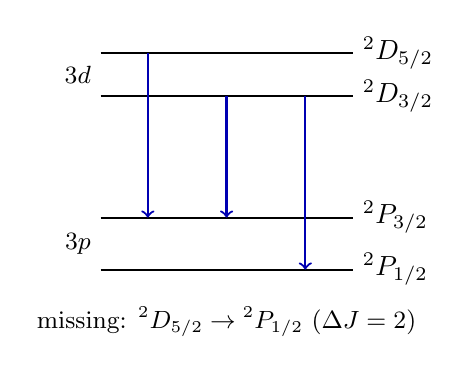
\begin{tikzpicture}[x=1cm,y=0.55cm]
\draw[thick] (0,6) -- (3.2,6) node[right] {\({}^2D_{5/2}\)};
\draw[thick] (0,5) -- (3.2,5) node[right] {\({}^2D_{3/2}\)};
\draw[thick] (0,2.2) -- (3.2,2.2) node[right] {\({}^2P_{3/2}\)};
\draw[thick] (0,1) -- (3.2,1) node[right] {\({}^2P_{1/2}\)};
\draw[->,thick,blue!70!black] (0.6,6) -- (0.6,2.2);
\draw[->,thick,blue!70!black] (1.6,5) -- (1.6,2.2);
\draw[->,thick,blue!70!black] (2.6,5) -- (2.6,1);
\node[left] at (0,5.5) {\small \(3d\)};
\node[left] at (0,1.6) {\small \(3p\)};
\node[font=\small] at (1.6,-0.2) {missing: \({}^2D_{5/2}\to{}^2P_{1/2}\) (\(\Delta J=2\))};
\end{tikzpicture}
\end{center}

\subsubsection*{Land\'e \(g\)-factors}
\[
g_J=1+\frac{J(J+1)+S(S+1)-L(L+1)}{2J(J+1)}.
\]
\begin{center}
\begin{tabular}{@{}lcccc@{}}
\toprule
Level & \(L\) & \(S\) & \(J\) & \(g_J\) \\
\midrule
\({}^2D_{5/2}\) & 2 & 1/2 & 5/2 & \(6/5=1.2\) \\
\({}^2D_{3/2}\) & 2 & 1/2 & 3/2 & \(4/5=0.8\) \\
\({}^2P_{3/2}\) & 1 & 1/2 & 3/2 & \(4/3\approx 1.333\) \\
\({}^2P_{1/2}\) & 1 & 1/2 & 1/2 & \(2/3\approx 0.667\) \\
\bottomrule
\end{tabular}
\end{center}
Weak-field energies: \(E=E_{\mathrm{FS}}+g_J\mu_B B\, m_J\).

\subsubsection*{Anomalous Zeeman}
Take the strongest line \({}^2D_{5/2}\to{}^2P_{3/2}\).
Upper: 6 sublevels, spacing \(1.2\,\mu_B B\). Lower: 4 sublevels, spacing \(1.333\,\mu_B B\).
Selection \(\Delta m_J=0,\pm 1\):
\begin{itemize}
\item \(\pi\) (\(\Delta m_J=0\)): vertical arrows.
\item \(\sigma_\pm\) (\(\Delta m_J=\pm 1\)): arrows one step right/left.
\end{itemize}
Viewed \(\perp\mathbf{B}\): \(\pi\) linear \(\parallel\mathbf{B}\), \(\sigma\) linear \(\perp\mathbf{B}\).
Viewed along \(\mathbf{B}\): only \(\sigma\), circular; \(\pi\) is absent.

Repeat the same picture for the other two FS lines.

\subsubsection*{Paschen--Back (\(\mu_B B\gg E_{\mathrm{FS}}\))}
Decouple: good quantum numbers \(m_\ell,m_s\) with \(E=\mu_B B(m_\ell+2m_s)\).
Optical: \(\Delta m_\ell=0,\pm 1\), \(\Delta m_s=0\) (light does not flip spin). Then
\[
\Delta E=\mu_B B\,\Delta m_\ell \in \{-\mu_B B,\;0,\;+\mu_B B\}.
\]
Normal Lorentz triplet. Polarisation: \(\pi\) (\(\Delta m_\ell=0\)), \(\sigma_\pm\) (\(\Delta m_\ell=\pm 1\)). Residual SO merely weakly splits each of the three.

\subsection{Problem 10 --- LS terms for \(\ell_1=1\), \(\ell_2=2\) (nonequivalent)}
Nonequivalent, so Pauli does not kill terms.
\(L=|\ell_1-\ell_2|\ldots \ell_1+\ell_2=1,2,3\) \(\Rightarrow\) \(P,D,F\).
\(S=0,1\) \(\Rightarrow\) singlets and triplets.

\begin{center}
\small
\begin{tabular}{@{}lllll@{}}
\toprule
Term & \(L\) & \(S\) & \(J\) & Symbols \\
\midrule
singlet P & 1 & 0 & 1 & \({}^1P_1\) \\
singlet D & 2 & 0 & 2 & \({}^1D_2\) \\
singlet F & 3 & 0 & 3 & \({}^1F_3\) \\
triplet P & 1 & 1 & 0,1,2 & \({}^3P_0,{}^3P_1,{}^3P_2\) \\
triplet D & 2 & 1 & 1,2,3 & \({}^3D_1,{}^3D_2,{}^3D_3\) \\
triplet F & 3 & 1 & 2,3,4 & \({}^3F_2,{}^3F_3,{}^3F_4\) \\
\bottomrule
\end{tabular}
\end{center}

\subsection{Problem 11 --- Stern--Gerlach, potassium, \(P_2P_3\)}
K ground state \(4s\;{}^2S_{1/2}\): two beams, \(\mu_z=\pm\mu_B\).
\(T=700~\mathrm{K}\), \(\partial B_z/\partial z=10^3~\mathrm{T\,m}^{-1}\), \(L=0.1~\mathrm{m}\), \(\ell=1~\mathrm{m}\).

\textbf{Geometry.} Magnet of length \(L\) along the beam, then a field-free flight of length \(\ell\) to the plate. Spots \(P_2,P_3\) are the two components. (If your figure swaps the labels, swap \(L\leftrightarrow\ell\) in the last line.)

Force \(F_z=\mu_B\partial B_z/\partial z\), acceleration \(a=F_z/M\). Time in the magnet \(t_1=L/v\). Deflection at magnet exit \(\tfrac12 a t_1^2\), plus extra \(a t_1\cdot(\ell/v)\) during the drift:
\[
s=\frac{\mu_B}{M}\frac{\partial B_z}{\partial z}\,\frac{L}{v^2}\left(\ell+\frac{L}{2}\right).
\]
Most probable thermal speed \(v=\sqrt{2kT/M}\). Potassium: \(M=39.1\,\mathrm{u}=6.49\times 10^{-26}~\mathrm{kg}\).
\[
v=546~\mathrm{m\,s}^{-1},\qquad a=1.43\times 10^5~\mathrm{m\,s}^{-2}.
\]
\[
s=0.0504~\mathrm{m},\qquad P_2P_3=2s=10.1~\mathrm{cm}.
\]
If the figure takes \(\ell=1~\mathrm{m}\) as the magnet and \(L=0.1~\mathrm{m}\) as the drift: \(2s\approx 58~\mathrm{cm}\). Quote the geometry you drew. The physically typical SG deflection with a 10~cm magnet is the 10~cm answer.

Traps: using \(J=3/2\) (excited K) \(\to\) 4 spots. Using \(g=1\) instead of \(g=2\) for \({}^2S_{1/2}\). Trying to do SG on electrons.

\subsection{Problem 12 --- Linear Stark of H, \(n=3\), and \(n=3\to 2\)}
Parabolic formula
\[
\Delta E=\frac32 n(n_1-n_2)\,e a_0\,\mathcal{E},\qquad
n=n_1+n_2+|m|+1.
\]

\textbf{\(n=3\) (9 orbital states \(\to\) 5 energies)}

\begin{center}
\small
\begin{tabular}{@{}cccccc@{}}
\toprule
\(n_1\) & \(n_2\) & \(m\) & \(n_1-n_2\) & \(\Delta E/(e a_0\mathcal{E})\) & degeneracy \\
\midrule
2 & 0 & 0 & \(+2\) & \(+9\) & 1 \\
1 & 0 & \(\pm 1\) & \(+1\) & \(+9/2\) & 2 \\
1 & 1 & 0 & 0 & 0 & 1 \\
0 & 0 & \(\pm 2\) & 0 & 0 & 2 \\
0 & 1 & \(\pm 1\) & \(-1\) & \(-9/2\) & 2 \\
0 & 2 & 0 & \(-2\) & \(-9\) & 1 \\
\bottomrule
\end{tabular}
\end{center}
Five levels: \(\pm 9,\;\pm 9/2,\;0\) (units \(e a_0\mathcal{E}\)). Degeneracies 1, 2, 3, 2, 1.
\(n=2\): three levels, \(\Delta E=0,\pm 3\,e a_0\mathcal{E}\).

\begin{center}
\begin{tikzpicture}[x=1.1cm,y=0.28cm]
\foreach \y/\lab in {9/+9, 4.5/+9/2, 0/0, -4.5/-9/2, -9/-9} {
  \draw[thick] (0,\y) -- (2.2,\y);
  \node[right] at (2.25,\y) {\small \(\lab\)};
}
\node[left] at (0,9) {\small \(n=3\)};
\foreach \y/\lab in {3/+3, 0/0, -3/-3} {
  \draw[thick] (4.2,\y) -- (6.4,\y);
  \node[right] at (6.45,\y) {\small \(\lab\)};
}
\node[left] at (4.2,3) {\small \(n=2\)};
\draw[->,blue!70!black] (2.2,0) -- (4.2,0);
\draw[->,blue!70!black] (2.2,4.5) -- (4.2,3);
\draw[->,red!70!black] (2.2,4.5) -- (4.2,0);
\node[font=\scriptsize,blue!70!black] at (3.2,-11.2) {\(\pi\): \(\Delta m=0\); \(\sigma\): \(\Delta m=\pm 1\)};
\end{tikzpicture}
\end{center}

E1: \(\Delta m=0\) (\(\pi\), \(\mathbf{E}_{\mathrm{light}}\parallel\boldsymbol{\mathcal{E}}\)) and \(\Delta m=\pm 1\) (\(\sigma\)).
The pattern is symmetric about the unshifted line (linear Stark). Draw the five \(n=3\) and three \(n=2\) bars, \(\pi\) arrows in the same-\(m\) column, \(\sigma\) arrows with \(\Delta m=\pm 1\).

\subsection{Problem 13 --- Pt ground term, \(\mu\), weak-field span}
Configuration: \([\mathrm{Xe}]\,4f^{14}5d^9 6s^1\). Closed \(4f^{14}\) is inert.
Treat \(5d^9\) as a \(d\)-\textbf{hole} (\(L=2,S=1/2\)) plus \(6s^1\) (\(l=0,s=1/2\)):
\[
L=2,\qquad S=0\text{ or }1 \quad\Rightarrow\quad {}^1D\text{ and }{}^3D.
\]
Hund: max \(S\) first \(\Rightarrow\) triplet \({}^3D\) is lower. The \(d^9\) shell is more than half full \(\Rightarrow\) inverted FS: highest \(J\) lies lowest.
\[
J=3,2,1 \quad\Rightarrow\quad \text{GS }={}^3D_3.
\]
\[
g_J=1+\frac{12+2-6}{2\cdot 12}=1+\frac{8}{24}=\frac43.
\]
\[
\mu=g_J\sqrt{J(J+1)}\,\mu_B=\frac43\sqrt{12}\,\mu_B=\frac{8\sqrt{3}}{3}\,\mu_B\approx 4.619\,\mu_B.
\]
Weak field: \(E=g_J\mu_B B m_J\), \(m_J=-3,\ldots,+3\). Extreme components \(\Delta m_J=6\):
\[
\Delta E_{\mathrm{span}}=6\cdot\frac43\cdot\mu_B B=8\,\mu_B B.
\]

\subsection{Problem 14 --- jj coupling, \((5/2)^4\)}
Four equivalent electrons in a \(j=5/2\) subshell. The subshell holds \(2j+1=6\) electrons, so \((5/2)^4\) is two \textbf{holes} in a closed \(j=5/2\) shell.
Two equivalent \(j=5/2\) fermions: Pauli \(\Rightarrow\) only even \(J\),
\[
J=0,2,4.
\]
Hole--particle symmetry: \((5/2)^4\) has the same list as \((5/2)^2\).
NIST: \((5/2)^2\) and \((5/2)^4\): \(J=0,2,4\).

\subsection{Problem 15 --- Helium \(\lvert\downarrow\downarrow\rangle\) is an eigenstate of \(S^2\) and \(S_z\)}
Two-electron spin-down product
\[
\chi=\lvert\beta(1)\beta(2)\rangle.
\]
\(\mathbf{S}=\mathbf{S}_1+\mathbf{S}_2\), \(\mathbf{S}_i=(\hbar/2)\boldsymbol{\sigma}_i\).

\textbf{\(S_z\).} \(\sigma_z\beta=-\beta\), so
\[
S_z\chi=\frac{\hbar}{2}(\sigma_{z1}+\sigma_{z2})\chi=-\hbar\,\chi.
\]
Eigenvalue \(-\hbar\) \(\Rightarrow\) \(M_S=-1\).

\textbf{\(S^2\).} Use \(S^2=S_1^2+S_2^2+2\mathbf{S}_1\cdot\mathbf{S}_2\) with \(S_i^2=(3/4)\hbar^2\) and
\[
\mathbf{S}_1\cdot\mathbf{S}_2=\frac{\hbar^2}{4}\,\boldsymbol{\sigma}_1\cdot\boldsymbol{\sigma}_2.
\]
Act on \(\chi=\lvert\downarrow\downarrow\rangle\):
\[
\begin{aligned}
\sigma_x\lvert\downarrow\rangle&=\lvert\uparrow\rangle
 &&\Rightarrow\; \sigma_{x1}\sigma_{x2}\chi=\lvert\uparrow\uparrow\rangle,\\
\sigma_y\lvert\downarrow\rangle&=-i\lvert\uparrow\rangle
 &&\Rightarrow\; \sigma_{y1}\sigma_{y2}\chi=-\lvert\uparrow\uparrow\rangle,\\
\sigma_z\lvert\downarrow\rangle&=-\lvert\downarrow\rangle
 &&\Rightarrow\; \sigma_{z1}\sigma_{z2}\chi=+\chi.
\end{aligned}
\]
\[
\boldsymbol{\sigma}_1\cdot\boldsymbol{\sigma}_2\,\chi=\lvert\uparrow\uparrow\rangle-\lvert\uparrow\uparrow\rangle+\chi=\chi.
\]
Hence \(\mathbf{S}_1\cdot\mathbf{S}_2\,\chi=(\hbar^2/4)\chi\), and
\[
S^2\chi=\Bigl(\tfrac34+\tfrac34+\tfrac12\Bigr)\hbar^2\chi=2\hbar^2\chi=1(1+1)\hbar^2\chi.
\]
So \(\chi\) is \(\lvert S=1,M_S=-1\rangle\), a triplet function, simultaneous eigenstate of \(S^2\) and \(S_z\).

\subsection{Problem 16 --- Li valence levels vs H}
Quantum defects: \(\delta_s=0.4\), \(\delta_p=0.04\), \(\delta_d=\delta_f=0\).
\[
E_{n\ell}(\mathrm{Li})=-13.6~\mathrm{eV}/(n-\delta_\ell)^2,\qquad
E_n(\mathrm{H})=-13.6~\mathrm{eV}/n^2.
\]
Effective quantum numbers for Li: \(n_s^*=n-0.4\), \(n_p^*=n-0.04\), \(n_{d,f}^*=n\).

\begin{center}
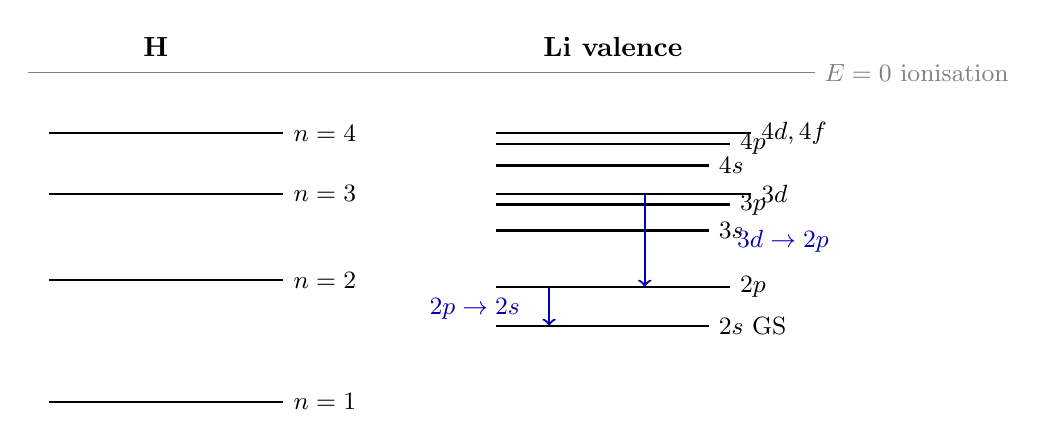
\begin{tikzpicture}[x=1.35cm, y=0.55cm]
\node at (1,8.6) {\textbf{H}};
\node at (5.3,8.6) {\textbf{Li valence}};
\draw[gray] (-0.2,8) -- (7.2,8) node[right] {\small \(E=0\) ionisation};
% H
\draw[thick] (0,6.6) -- (2.2,6.6) node[right] {\small \(n=4\)};
\draw[thick] (0,5.2) -- (2.2,5.2) node[right] {\small \(n=3\)};
\draw[thick] (0,3.2) -- (2.2,3.2) node[right] {\small \(n=2\)};
\draw[thick] (0,0.4) -- (2.2,0.4) node[right] {\small \(n=1\)};
% Li
\draw[thick] (4.2,6.6) -- (6.6,6.6) node[right] {\small \(4d,4f\)};
\draw[thick] (4.2,6.35) -- (6.4,6.35) node[right] {\small \(4p\)};
\draw[thick] (4.2,5.85) -- (6.2,5.85) node[right] {\small \(4s\)};
\draw[thick] (4.2,5.2) -- (6.6,5.2) node[right] {\small \(3d\)};
\draw[thick] (4.2,4.95) -- (6.4,4.95) node[right] {\small \(3p\)};
\draw[thick] (4.2,4.35) -- (6.2,4.35) node[right] {\small \(3s\)};
\draw[thick] (4.2,3.05) -- (6.4,3.05) node[right] {\small \(2p\)};
\draw[thick] (4.2,2.15) -- (6.2,2.15) node[right] {\small \(2s\) GS};
\draw[->,thick,blue!70!black] (4.7,3.05) -- (4.7,2.15);
\draw[->,thick,blue!70!black] (5.6,5.2) -- (5.6,3.05);
\node[font=\small,blue!70!black] at (4.0,2.55) {\(2p\to 2s\)};
\node[font=\small,blue!70!black] at (6.9,4.1) {\(3d\to 2p\)};
\end{tikzpicture}
\end{center}

Forbidden: \(3s\to 2s\) (\(\Delta\ell=0\)), \(3d\to 2s\) (\(\Delta\ell=2\)). Li \(1s^2\) is a filled core, not the valence.

\subsection{Problem 17 --- Unsold's theorem, prove for \(\ell=1\)}
\textbf{Statement.} For a filled \(\ell\)-subshell (or the sum over \(m\) at fixed \(\ell\)),
\[
\sum_{m=-\ell}^{\ell}\lvert Y_{\ell m}(\theta,\phi)\rvert^2=\frac{2\ell+1}{4\pi},
\]
independent of angle. The charge density of a closed subshell is spherically symmetric.

\textbf{Proof, \(\ell=1\), using the given \(\Phi,\Theta\).}
\[
\Phi=\frac{1}{\sqrt{2\pi}},\qquad
\Theta_{10}=\frac{\sqrt{6}}{2}\cos\theta,\qquad
\Theta_{1\pm 1}=\frac{\sqrt{3}}{2}\sin\theta.
\]
\[
\lvert Y_{10}\rvert^2=\frac{3}{4\pi}\cos^2\theta,\qquad
\lvert Y_{1\pm 1}\rvert^2=\frac{3}{8\pi}\sin^2\theta.
\]
\[
\sum_{m=-1}^{1}\lvert Y_{1m}\rvert^2
=\frac{3}{4\pi}\cos^2\theta+2\cdot\frac{3}{8\pi}\sin^2\theta
=\frac{3}{4\pi}(\cos^2\theta+\sin^2\theta)
=\frac{3}{4\pi}
=\frac{2\cdot 1+1}{4\pi}.
\]
Independent of \(\theta\) and \(\phi\).

\subsection{Problem 18 --- True / False}
\textbf{All seven statements are FALSE.}

\begin{enumerate}[leftmargin=1.4em]
\item At small \(r\), for \(\ell\neq 0\), \(R_{nl}\propto r^{\ell+1}\).
\textbf{FALSE.} \(R_{nl}\propto r^{\ell}\). It is \(u(r)=r R_{nl}\) that goes as \(r^{\ell+1}\).
\item Series limit of Lyman of H lies in the visible.
\textbf{FALSE.} Lyman limit is \(91.2~\mathrm{nm}\), vacuum UV.
\item Stimulated-emission rates are independent of the intensity of the incident radiation.
\textbf{FALSE.} Stimulated rate \(=B_{21}\rho(\nu)\). Spontaneous \(A_{21}\) is the intensity-independent one.
\item In alkali atoms \(\ell\)-degeneracy is removed because the effective potential is not spherically symmetric.
\textbf{FALSE.} The central-field potential \textbf{is} spherically symmetric (that is why \(m\) remains degenerate). \(\ell\)-degeneracy dies because \(V_{\mathrm{eff}}\) is not Coulomb \(1/r\).
\item The energy of an Auger electron depends on the energy of the radiation which created the initial vacancy.
\textbf{FALSE.} \(K_{\mathrm{Auger}}=E_{\mathrm{hole}}-E_{\mathrm{filler}}-E_{\mathrm{ejected}}\). Photoelectrons \emph{do} remember the photon; Auger electrons do not.
\item Atomic transitions forbidden under the dipole approximation are `strictly forbidden'.
\textbf{FALSE.} They proceed by M1, E2, two-photon decay, collisions, \ldots Strictly forbidden is reserved for exact-symmetry bans (e.g.\ \(J=0\to 0\)).
\item Electrons in high Rydberg states are very strongly bound.
\textbf{FALSE.} \(E_b=13.6~\mathrm{eV}/n^2\to 0\). They are weakly bound.
\end{enumerate}
The two people miss under exam stress are (i) (confusing \(R\) with \(u\)) and (iv) (confusing spherical with Coulomb).

\newpage
%======================================================================
\section{Last-hour drill}
%======================================================================

Read this once in the morning. Do not open a textbook.

\subsection*{60-second constants}
\[
R_\infty=109737~\mathrm{cm}^{-1},\quad R_H=109678~\mathrm{cm}^{-1},\quad 13.6~\mathrm{eV},\quad a_0=0.529~\text{\AA}
\]
\[
R_M=R_\infty/(1+m_e/M),\quad m_p/m_e=1836,\quad M_D/m_e=3670
\]
Na \(D_2=589.0~\mathrm{nm}=3\,{}^2P_{3/2}\to 3\,{}^2S_{1/2}\). \(D_1=589.6~\mathrm{nm}\).

\subsection*{Diagrams you must be able to draw blind}
\begin{enumerate}
\item H series. Lyman UV, Balmer vis, rest IR. Overlap starts at Paschen/Brackett.
\item Li vs H. \(ns\) pulled down (\(\delta=0.4\)), \(np\) a little (\(\delta=0.04\)), \(nd,nf\) on H. Arrows: \(2p\to 2s\), \(3d\to 2p\).
\item Na \(3d\to 3p\) FS. Three lines. Missing \({}^2D_{5/2}\to{}^2P_{1/2}\).
\item Anomalous Zeeman of a doublet (Na D): \({}^2P_{3/2}\) (4), \({}^2P_{1/2}\) (2), \({}^2S_{1/2}\) (2). \(\pi\) \(\Delta m=0\), \(\sigma\) \(\Delta m=\pm 1\).
\item Paschen--Back. \(E=\mu_B B(m_L+2m_S)\). Triplet. \(\Delta m_S=0\).
\item Stark \(n=3\). Five bars at \(0,\pm 4.5,\pm 9\) (\(e a_0\mathcal{E}\)). \(n=2\): three bars at \(0,\pm 3\).
\item SG. Two spots for \({}^2S_{1/2}\). \(F_z=\mu_z\partial B_z/\partial z\). Not for free \(e^-\).
\end{enumerate}

\subsection*{\(g_J\) flash}
\[
g=1+\frac{J(J+1)+S(S+1)-L(L+1)}{2J(J+1)}
\]
\({}^2S_{1/2}\to 2\), \({}^2P_{1/2}\to 2/3\), \({}^2P_{3/2}\to 4/3\), \({}^2D_{3/2}\to 4/5\), \({}^2D_{5/2}\to 6/5\), singlets \(\to 1\).

\subsection*{Widths}
Natural (mean life \(\tau\), lower level stable): \(\Delta\nu=1/(2\pi\tau)\). Na \(16~\mathrm{ns}\Rightarrow 10~\mathrm{MHz}\).\\
Doppler FWHM: \(\Delta\lambda=(2\lambda/c)\sqrt{2kT\ln 2/M}\). Scales \(\sqrt{T/M}\,\lambda\).\\
Stimulated \(\propto I\). Spontaneous does not.

\subsection*{Scaling laws}
\begin{center}
\begin{tabular}{@{}ll@{}}
\toprule
Quantity & Scale \\
\midrule
Bohr energy & \(\mu Z^2/n^2\) \\
Bohr radius & \(n^2/\mu Z\) \\
Fine-structure interval & \(Z^4/[n^3\ell(\ell+1)]\) \\
Linear Stark & \(n(n_1-n_2)e a_0\mathcal{E}\) \\
Weak Zeeman & \(g_J\mu_B B m_J\) \\
Rydberg spacing & \(27.2~\mathrm{eV}/n^3\) \\
Exciton Rydberg & \(13.6\,(\mu/m_e)/\varepsilon_r^2\) \\
\bottomrule
\end{tabular}
\end{center}

\subsection*{Five exam traps (the difference between 90 and 100)}
\begin{enumerate}
\item \textbf{Reduced mass.} Any mention of D, \(\mu\), \(\pi\), or \(R_\infty\) vs \(R_H\) is a reduced-mass question.
\item \(Z^4\) for fine structure, \(Z^2\) for Bohr energies, \(1/n^3\) for Rydberg spacings and SO.
\item \(\Delta J=2\) is E1-forbidden. Count lines before drawing them.
\item Geometry of SG. Write \(s=\frac{\mu}{M}(\partial B/\partial z)(L/v^2)(\ell+L/2)\) and \(2s\). State which length is the magnet.
\item Spherical \(\neq\) Coulomb. \(m\)-degeneracy from spherical; \(\ell\)-degeneracy from \(1/r\).
\end{enumerate}

\subsection*{If a derivation is asked}
\textbf{Rydberg from correspondence.} Classical \(E(\omega)\) + \(\omega=4\pi Rc/n^3\) \(\Rightarrow R_\infty=me^4/(8\varepsilon_0^2 h^3 c)\).\\
\textbf{SG force.} \(U=-\mu\cdot B\Rightarrow F_z=\mu_z\partial B_z/\partial z\). Drop \(F_x,F_y\).\\
\textbf{SO.} \(\mathbf{B}_L\propto\mathbf{L}/r^3\), Thomas 1/2, \(\mathbf{L}\cdot\mathbf{S}=\tfrac12(J^2-L^2-S^2)\), \(\langle r^{-3}\rangle\propto Z^3/[n^3\ell(\ell+1/2)(\ell+1)]\).\\
\textbf{Dipole \(\Delta m\).} \(z\Rightarrow\int e^{i(m_a-m_b)\phi}d\phi\Rightarrow\Delta m=0\); \(x\pm iy\Rightarrow\Delta m=\pm 1\). Parity of \(Y_{\ell m}\) is \((-1)^\ell\).

\vspace{1.2em}
\begin{center}
\textit{That is the whole quiz. Draw the diagrams once more, then sleep.}
\end{center}

\end{document}
